\chapter{Production Plan}
\label{ch:ProductionPlan}
This chapter describes the proposed production plan for the eVTOL under analysis. 
Particularly, a comparison between in-house production and outsourcing will be held, specifying for each subsystem the chosen production method.
Finally, the production line and its timeline will be described.

\section{Comparison between Vertical and Horizontal Integration}
During the manufacturing process of a system as complex as an aircraft, customised and high-quality parts are likely needed.
These parts can either be produced in-house (vertical integration) or purchased/commissioned by specialised contractors (horizontal integration). An example of these methods in the eVTOL industry are Joby \cite{jobyaviation} and Archer aviation \cite{archer_evtolnews} relatively.

Joby has opted for a vertical integration model, claiming that this leads to a more optimised product overall, designed for the specific application.
On the other hand, Archer Aviation has opted for a horizontal integration model, outsourcing more than 80\% of its components \cite{integration}.
The advantages that this brings, according to the company, are lower initial investments and a smoother entry into the market, as several subsystems from suppliers already possess certifications.
From this competition philosophy analysis, the two methods can be further analysed, as will be done in this section.

Self-manufacturing brings several advantages, especially in the context of serial production.
Particularly in the aerospace industry, intellectual property and innovation represent key pillars. This implies that it is safer to restrict access of sub-competitors to technical details of innovations, shielding the design from competitors.
For instance, the hinge mechanism used in this project is a proprietary technology, thus producing it in-house reduces the risk of specifications being leaked to the competitors.

Another reason for which self-production could be adopted is for quality control purposes.
It is indeed easier to directly manage the quality of each product when developed in-house rather than when obtained from a sub-contractor.
An example of this issue is the accident that occurred in January 2024 on board a Boeing 737-MAX, where the door blew out mid-flight~\cite{incident}.
The door handle was manufactured by a subcontractor, and several quality-related flaws have been identified.
Certainly, quality assurance could be performed on the subcontractor component as well, but the self-production of the subsystem guarantees more control over the product.
Quality control might not be relevant in the initial stage of production considering the small size of the team. However, it can become a major issue as the production scales up.

One last parameter to be taken into consideration when deciding between self-production and commissioning are the supply-chain risks.
When commissioning, each part could prove critical and cause several delays in the manufacturing process of the whole product. Thus, one contractor delivering the product late might delay the entire production line, generating enormous economic losses.

On the other hand, outsourcing the production of some parts does bring advantages.
Firstly, for the production of some elements, where highly specific machines are required, starting completely new production lines comes with major costs.
In addition to this, subcontractors often specialise in a specific technological area, meaning that they can deliver high-quality products that are in line with the requirements.
For example, in the case of propulsion units, it turns out to be much cheaper to acquire engines from external sources, rather than spend substantial economic and time resources on the research, development, and production of such a component.
Lastly, purchasing some elements of the assembly could benefit scalability.
This is particularly relevant when a higher production rate is needed, it is easier for a specialised company to produce larger batches of certain components, due to the high likelihood that the facility's manufacturing capabilities are ensured.
This concept is valid when considering a slowdown in production as well, which could be caused by lower demand or external factors.
Purchasing parts from external contractors implies ordering fewer parts from them, while in the case of self-production, it would potentially lead to shutting down factories and firing employees.

\section{Production Method per Subsystem}
After understanding the main criteria that determine whether in-house production or commissioning is the best option, it is possible to draw some initial conclusions.
For each sub-system, several criteria are considered as shown in \Cref{tab:prodcriteria}.

\begin{table}[ht]
\centering
\caption{Criteria to evaluate in-house production and outsourcing}
\label{tab:prodcriteria}
\begin{tabular}{lll}
\toprule
\textbf{ID} & \textbf{Criterion} & \textbf{Description}                                                                            \\ \midrule
\textit{PR-01}       & Costs                          & \begin{tabular}[c]{@{}l@{}} Costs related to the production \end{tabular}                                                  \\ 
\textit{PR-02}       & Expertise needed             & \begin{tabular}[c]{@{}l@{}}Specific knowledge and expertise needed about the technology
\end{tabular}                                                           \\ 
\textit{PR-03}       & Quality control       & \begin{tabular}[c]{@{}l@{}} Expected product quality from the production\end{tabular} \\ 
\textit{PR-04}       & Secretive technology                        & \begin{tabular}[c]{@{}l@{}}Novelty of the technology and if it needs\\ to be hidden from competition \end{tabular}                                                                                        \\ 
\textit{PR-05}       & Supply Chain                      & \begin{tabular}[c]{@{}l@{}} Supply chain dependency and availability \end{tabular}               \\ 
\textit{PR-06}       & Scalability               & \begin{tabular}[c]{@{}l@{}} Ease to scale-up and scale down\end{tabular}                              \\ \bottomrule
\end{tabular}
\end{table}

All of these criteria are evaluated for each subsystem and a trade-off is performed, establishing which of the two production methodologies would be more advantageous.
The trade-off, in this case, is conducted in a different manner than the one performed for the design choice in \Cref{ch:TradeOff}.
This is because some criteria have different weights for different subsystems.
For example, for a new technology, protecting intellectual property from competition is the driving criterion while for the production of a common bolt, it is not.
Thus, this trade-off has been performed case by case listing the advantages and disadvantages of the two choices, resulting in the decisions that can be seen in the following table:

\begin{table}[ht]
\centering
\caption{Subsystem production method}
\label{prod2}
\begin{tabular}{p{3.2cm}cp{6.5cm}l}
\toprule
\textbf{Subsystem}                          & \textbf{Method} & \textbf{Reasoning}                                                                      & \textbf{Possible Supplier} \\ \midrule
{Propulsion}                                                            & {Outsource}                               & {Very high development costs and specific knowledge needed}               & {Safran Aircraft Engines}                            \\ \hline
{Landing gear}                                                          & {Outsource}                               & {Not very specific component that has been produced by several companies} & {Lierbherr}                                          \\ \hline
{Fuselage}                                                             & {In-house}                                & {High-quality control needed and supply chain stability}                  & {N.A.}                                                \\ \hline
{Hinge mechanism}            & {In-house}                                & {Protect intellectual property on a novel technology}                     & {N.A.}                                                \\ \hline
{Battery}                                                               & {Outsource}                               & {High-performance product that only a few companies produce}             & {InoBat}                                             \\ \hline
{Electronics and wiring}     & {Outsource}                               & {Several suppliers offer off the shelf products}                          & {Collins Aerospace}                                  \\ \hline
{Autonomous system}           & {Outsource}                               & {Several specialised companies already in the market}                     & {Collins Aerospace}                                  \\ \hline
{Wings and Control surfaces} & {In-house}                                & {High-quality control needed and supply chain stability}                  & {N.A.}                                                \\ \hline
{Bolts, fasteners...}                                                   & {Outsource}                               & {Several suppliers offer off the shelf products}                          & {TriMas Aerospace}                                   \\ \bottomrule
\end{tabular}
\end{table}

In \Cref{prod2} a list of possible suppliers is compiled.
This is just an indication of the companies from which parts could be acquired, but these choices are susceptible to change during the detailed design phase.
To prevent strong dependencies on a single supplier the desired contractor list has been diversified.
It is important to consider that in this stage of the design, the production plan's resolution focuses on the subsystems, but this could be shifted to the individual parts as the product design advances.
Moreover, as of yet, the manufacturing process for the self-produced parts has still not been determined.
Once these choices are made, more information about the manufacturing process will be provided.

\section{Assembly Line}
As soon as the necessary components of the eVTOL have been produced or purchased, the assembly of the final product can start.
First of all, each of the subsystems needs to be assembled in the subassembly lines.
The subassemblies then leave one line to enter another one, until reaching the station in which the subsystem is assembled.
For example, the wing is composed of several subassemblies that are first assembled in their own stations and then joined up in the final wing line.

At this point of the production phase, the final aircraft assembly can start.
Once the fuselage parts are joined, all the subsystems can be mounted on the vehicle, until the final product state is reached.
It is important to note that this process needs optimisation and coordination of different departments in the same factory, in order to achieve time- and cost-efficient production.

Another important aspect to take into consideration is performing quality control during the whole manufacturing and assembly process.
Quality assurance needs to be thoroughly ensured at each station, for each subassembly, so as to identify and correct any flaw as early as possible during the production phase.
The final assembly process can be visualised in the following figure as a timeline :
\begin{figure}[ht]
    \centering
    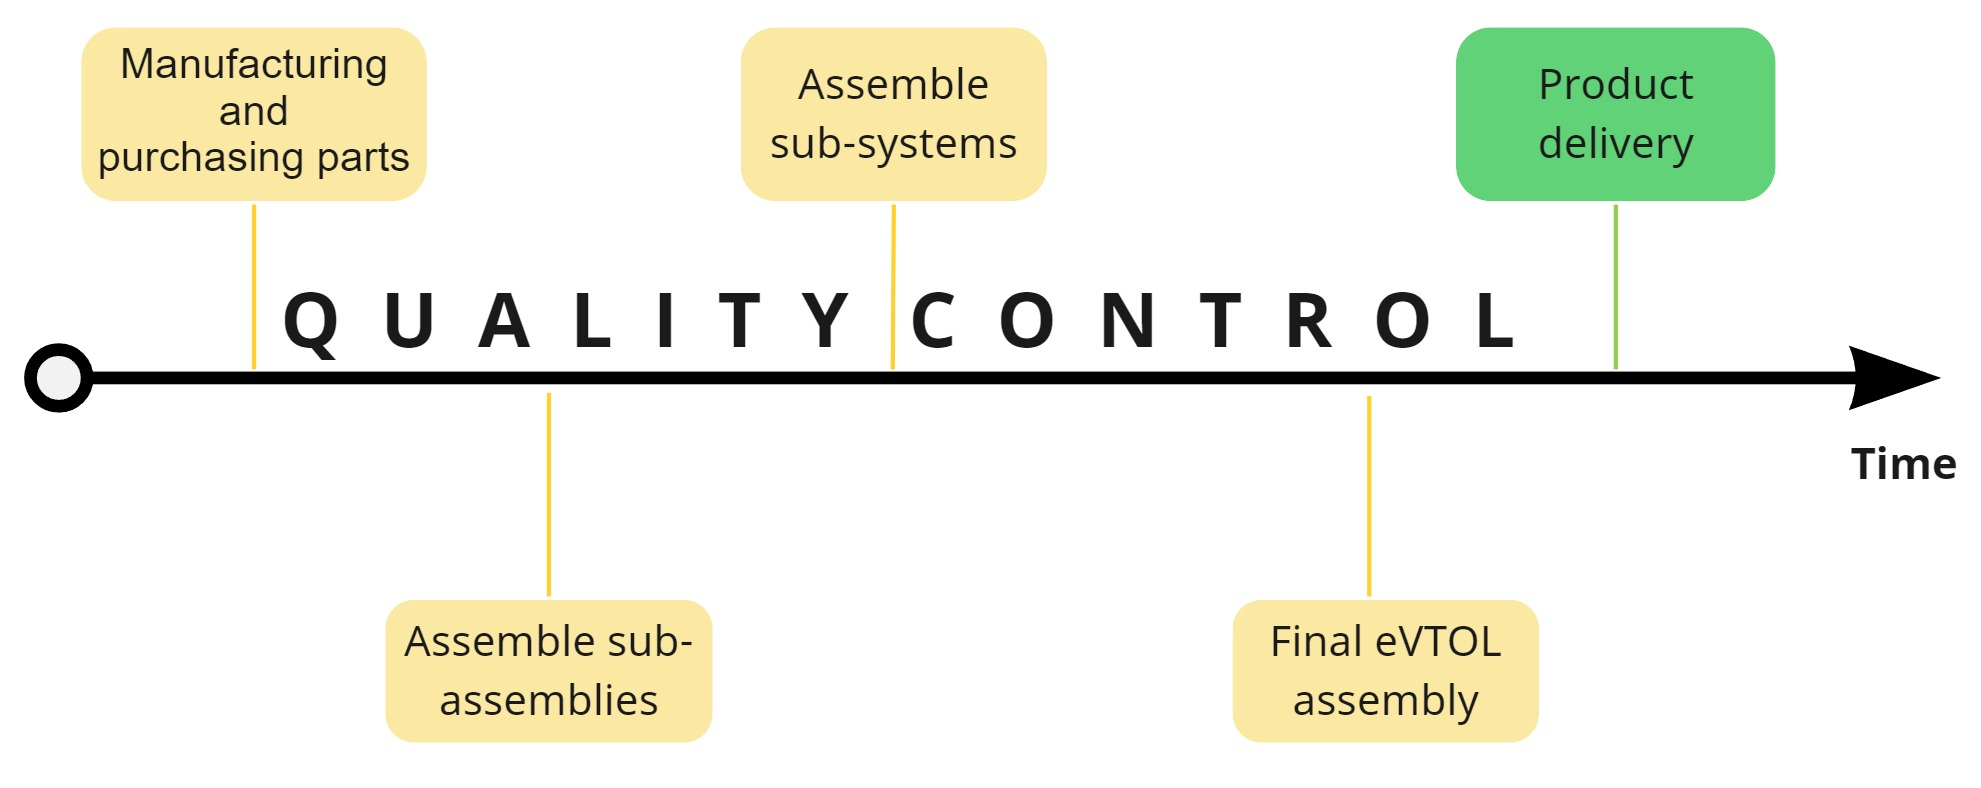
\includegraphics[width=\linewidth]{figures/Timeline.jpg}
    \caption{Production timeline}
    \label{fig:timeline}
\end{figure}

\Cref{fig:timeline} defines visually how the production process will develop over time.
It is noticeable how the time span is not indicated, due to the fact that at this stage of the design process, the time required for performing each of the phases has not been defined.
Lastly, more detailed information will be added to the timeline as soon as the manufacturing methods are chosen.

